% Persönliche Informationen (für die Titelseite und den Footer)

\title[Rubik's Cube-Workshop]{Rubik's Cube-Workshop}
\author{Jan Dillmann}
\institute{\href{http://www.jandillmann.de}{www.jandillmann.de}}
\subject{Rubik's Cube}
\keywords{Rubik's Cube, Tutorial, Zauberwürfel, Anfänger, Algorithmus}
\titlegraphic{%
	\begin{columns}[c]
		\begin{column}[T]{.5\textwidth}
			\center
			
\includegraphics[height=75pt]{img/solved2}
		\end{column}
		\begin{column}[T]{.5\textwidth}
			\center
			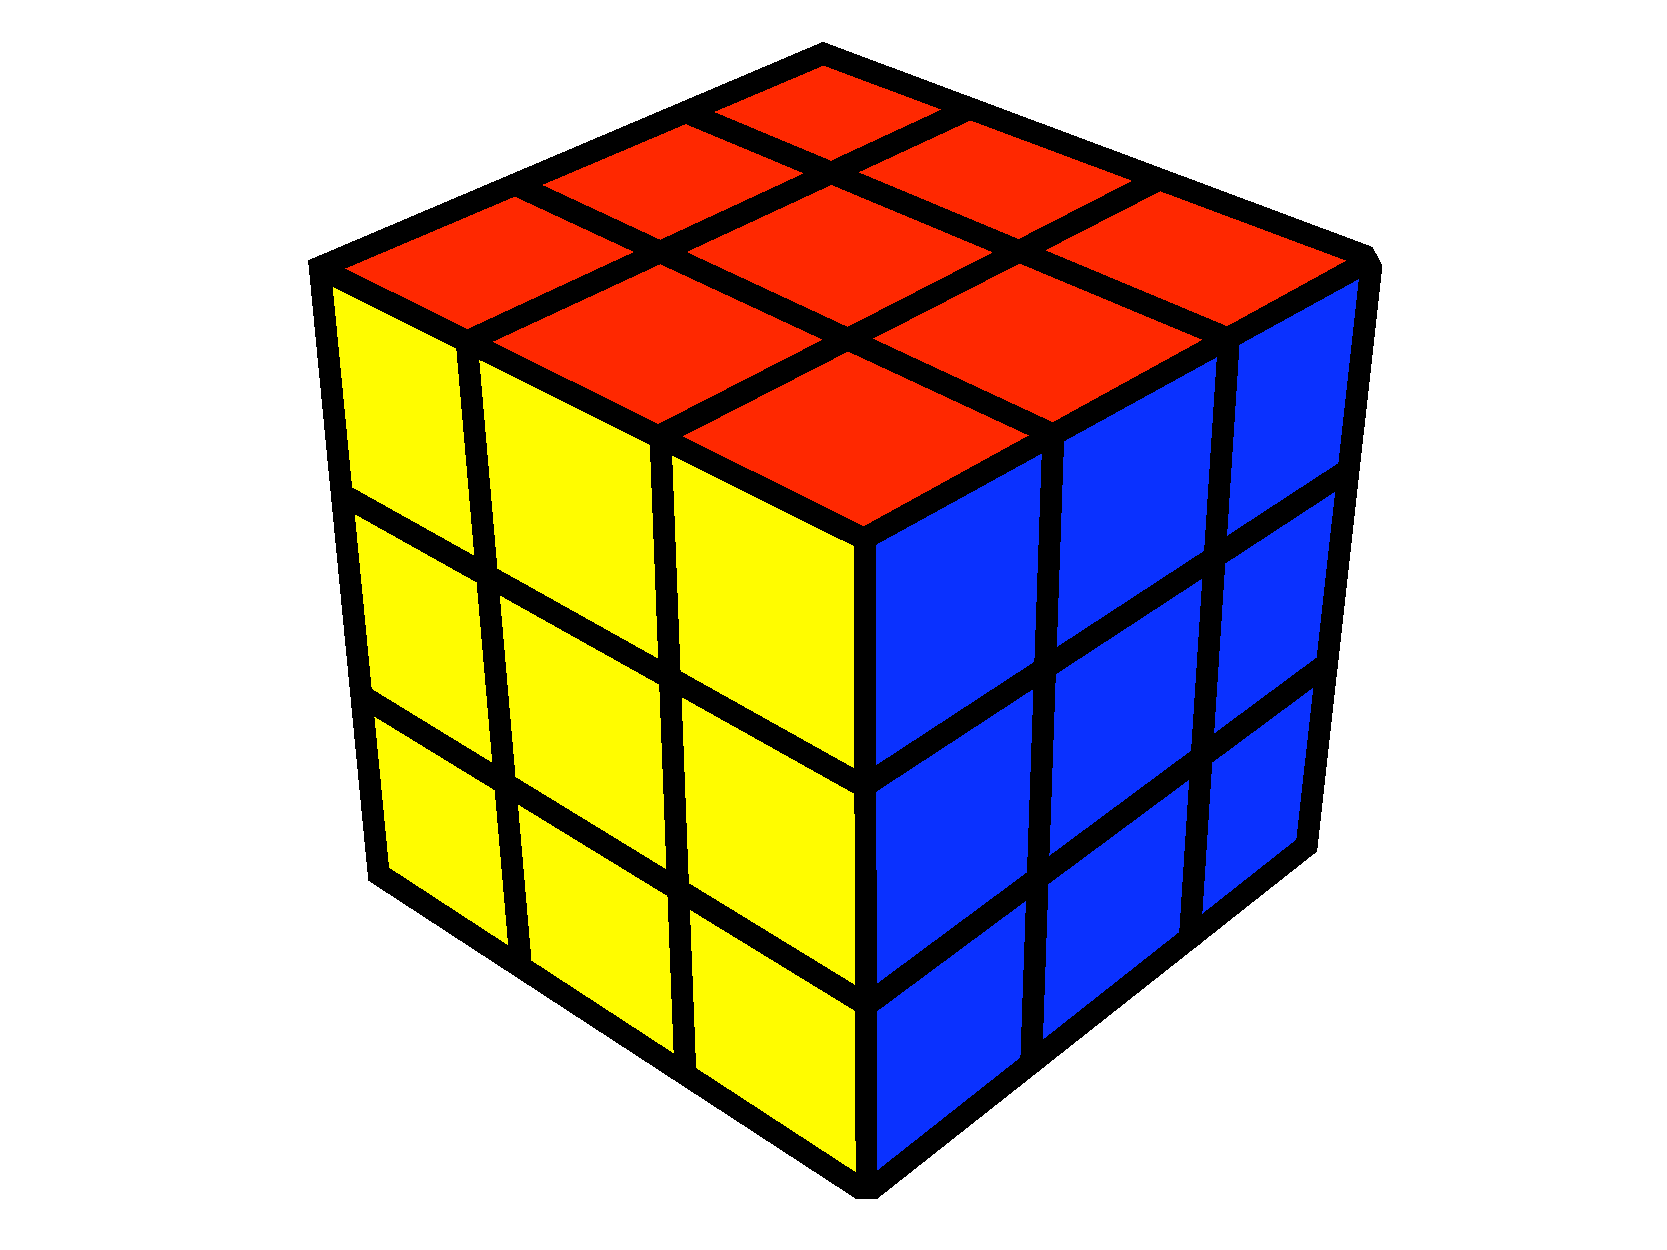
\includegraphics[height=75pt]{img/solved1}
		\end{column}
	\end{columns}
}
